\section{3D Bin Packing Problem}

\section{Support} %TODO: Here or in introduction?

\section{MILP Formulation}
\label{sec:milp}%
\subsection*{Conceptual model}
A conceptual model of the problem we are trying to solve would be:

%TODO: Cage Ratio?
\begin{align*}
    \textbf{minimize} \hspace{.5cm}   & \text{unused volume in used bins} \\
    \textbf{subject to} \hspace{.5cm} & \text{all items assigned to one and only one bin} \\
                                      & \text{all items within the bin dimensions} \\
                                      & \text{no overlaps between items in the same bin} \\
                                      & \text{all items with support} \\
\end{align*}

We can now provide the formal definition of the 3DBPP by formulating a mixed integer linear programming problem model.

\subsection*{Formal model}
\label{ssec:formal_model}
We'll now introduce a MILP model for the standard 3DBPP problem definition and then we'll expand it to address the stability constraint afterwards.

We start by defining the known sets and parameters of the problem.
\paragraph*{Sets}
\begin{align*}
    I = \{1,\dots, n \}: \hspace{.5cm}& \text{set of items} \\
    B = \{1,\dots, m \}: \hspace{.5cm}& \text{set of bins} 
\end{align*}
\paragraph*{Parameters}
\begin{align}
          W \times D \times H  \hspace{.5cm}& \text{width $\times$ depth $\times$ height of a bin} \notag \\
                            V  \hspace{.5cm}& \text{bin volume} \notag \\
    w_i \times d_i \times h_i  \hspace{.5cm}& \text{width $\times$ depth $\times$ height of item $i$} & \forall i \in I \label{par:item_dim}
\end{align}

\paragraph*{Variables} We can now introduce the following sets of integer variables
\begin{align}
              (x_i,y_i,z_i) \hspace{.5cm}& \text{bottom front left corner of an item} & \forall i \in I \label{var:item_pos} \\
                    v_{b} \hspace{.5cm}& \begin{cases}
                                            1, \text{if bin $b$ is used} \\ 
                                            0, \text{otherwise}
                                        \end{cases} & \forall i \in I, \forall b \in B \notag \\
                    u_{ib} \hspace{.5cm}& \begin{cases}
                                            1, \text{if item $i$ is placed in bin $b$} \\ 
                                            0, \text{otherwise}
                                        \end{cases} & \forall i \in I, \forall b \in B \notag \\
                    x^p_{ij} \hspace{.5cm}& \begin{cases}
                                            1, \text{if $x_i + w_i \le x_j$} \\ 
                                            0, \text{otherwise}
                                        \end{cases} & \forall i,j \in I \notag \\
                    y^p_{ij} \hspace{.5cm}& \begin{cases}
                                            1, \text{if $y_i + d_i \le y_j$} \\ 
                                            0, \text{otherwise}
                                        \end{cases} & \forall i,j \in I \notag \\
                    z^p_{ij} \hspace{.5cm}& \begin{cases}
                                            1, \text{if $z_i + h_i \le z_j$} \\ 
                                            0, \text{otherwise}
                                        \end{cases} & \forall i,j \in I \notag \\
            z_b^\text{max} \hspace{.5cm}& \text{maximum height of bin $b$} & \forall b \in B \notag
\end{align}

Given a coordinate system, each item $i$ can be represented univocally in 3D space by \cref{par:item_dim,var:item_pos} as seen in figure \ref{fig:coordinate_system}
\begin{figure}
    \scalebox{0.65}{%
    

\tikzset{every picture/.style={line width=0.75pt}} %set default line width to 0.75pt        

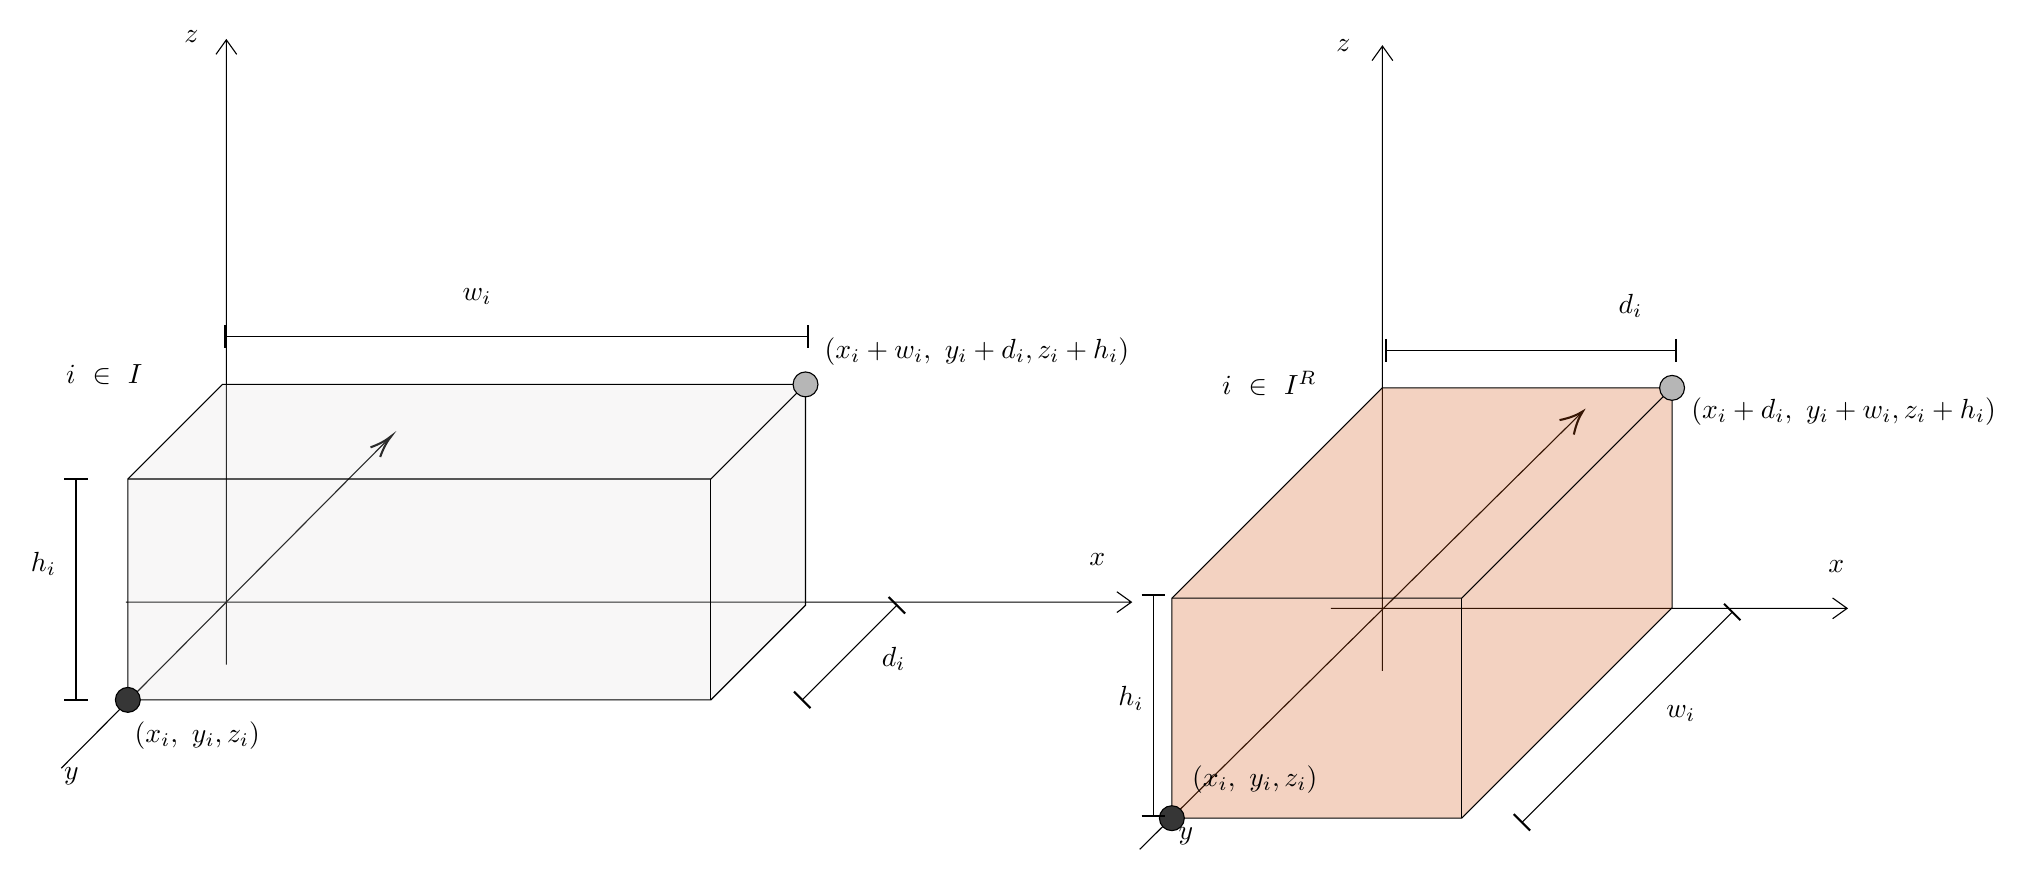
\begin{tikzpicture}[x=0.75pt,y=0.75pt,yscale=-1,xscale=1]
%uncomment if require: \path (0,479); %set diagram left start at 0, and has height of 479

%Shape: Axis 2D [id:dp17090047473688563] 
\draw  (122,295.9) -- (606.5,295.9)(170.45,25) -- (170.45,326) (599.5,290.9) -- (606.5,295.9) -- (599.5,300.9) (165.45,32) -- (170.45,25) -- (175.45,32)  ;
%Straight Lines [id:da9671294084497354] 
\draw    (248.54,217.32) -- (90.95,375.9) ;
\draw [shift={(249.95,215.9)}, rotate = 134.82] [color={rgb, 255:red, 0; green, 0; blue, 0 }  ][line width=0.75]    (10.93,-3.29) .. controls (6.95,-1.4) and (3.31,-0.3) .. (0,0) .. controls (3.31,0.3) and (6.95,1.4) .. (10.93,3.29)   ;
%Shape: Cube [id:dp18105788479145446] 
\draw  [fill={rgb, 255:red, 218; green, 217; blue, 217 }  ,fill opacity=0.2 ] (123,236.6) -- (168.6,191) -- (449.5,191) -- (449.5,297.4) -- (403.9,343) -- (123,343) -- cycle ; \draw   (449.5,191) -- (403.9,236.6) -- (123,236.6) ; \draw   (403.9,236.6) -- (403.9,343) ;
%Flowchart: Connector [id:dp700077731080137] 
\draw  [fill={rgb, 255:red, 54; green, 54; blue, 54 }  ,fill opacity=1 ] (117,343) .. controls (117,339.69) and (119.69,337) .. (123,337) .. controls (126.31,337) and (129,339.69) .. (129,343) .. controls (129,346.31) and (126.31,349) .. (123,349) .. controls (119.69,349) and (117,346.31) .. (117,343) -- cycle ;
%Flowchart: Connector [id:dp7959957780151166] 
\draw  [fill={rgb, 255:red, 182; green, 182; blue, 182 }  ,fill opacity=1 ] (443.5,191) .. controls (443.5,187.69) and (446.19,185) .. (449.5,185) .. controls (452.81,185) and (455.5,187.69) .. (455.5,191) .. controls (455.5,194.31) and (452.81,197) .. (449.5,197) .. controls (446.19,197) and (443.5,194.31) .. (443.5,191) -- cycle ;
%Straight Lines [id:da2736427434795695] 
\draw    (169.6,168) -- (450.5,168) ;
\draw [shift={(450.5,168)}, rotate = 180] [color={rgb, 255:red, 0; green, 0; blue, 0 }  ][line width=0.75]    (0,5.59) -- (0,-5.59)   ;
\draw [shift={(169.6,168)}, rotate = 180] [color={rgb, 255:red, 0; green, 0; blue, 0 }  ][line width=0.75]    (0,5.59) -- (0,-5.59)   ;
%Straight Lines [id:da5491305384137963] 
\draw    (447.9,343) -- (493.5,297.4) ;
\draw [shift={(493.5,297.4)}, rotate = 135] [color={rgb, 255:red, 0; green, 0; blue, 0 }  ][line width=0.75]    (0,5.59) -- (0,-5.59)   ;
\draw [shift={(447.9,343)}, rotate = 135] [color={rgb, 255:red, 0; green, 0; blue, 0 }  ][line width=0.75]    (0,5.59) -- (0,-5.59)   ;
%Straight Lines [id:da2096690092171385] 
\draw    (98,343) -- (98,236.6) ;
\draw [shift={(98,236.6)}, rotate = 90] [color={rgb, 255:red, 0; green, 0; blue, 0 }  ][line width=0.75]    (0,5.59) -- (0,-5.59)   ;
\draw [shift={(98,343)}, rotate = 90] [color={rgb, 255:red, 0; green, 0; blue, 0 }  ][line width=0.75]    (0,5.59) -- (0,-5.59)   ;
%Shape: Axis 2D [id:dp7776925959360946] 
\draw  (702.58,298.9) -- (951.33,298.9)(727.45,28) -- (727.45,329) (944.33,293.9) -- (951.33,298.9) -- (944.33,303.9) (722.45,35) -- (727.45,28) -- (732.45,35)  ;
%Straight Lines [id:da8573442295183169] 
\draw    (822.58,205.41) -- (610.5,415) ;
\draw [shift={(824,204)}, rotate = 135.34] [color={rgb, 255:red, 0; green, 0; blue, 0 }  ][line width=0.75]    (10.93,-4.9) .. controls (6.95,-2.3) and (3.31,-0.67) .. (0,0) .. controls (3.31,0.67) and (6.95,2.3) .. (10.93,4.9)   ;
%Shape: Cube [id:dp7879935806557912] 
\draw  [color={rgb, 255:red, 0; green, 0; blue, 0 }  ,draw opacity=1 ][fill={rgb, 255:red, 209; green, 82; blue, 15 }  ,fill opacity=0.26 ] (626,294) -- (727.33,192.67) -- (867,192.67) -- (867,298.67) -- (765.67,400) -- (626,400) -- cycle ; \draw  [color={rgb, 255:red, 0; green, 0; blue, 0 }  ,draw opacity=1 ] (867,192.67) -- (765.67,294) -- (626,294) ; \draw  [color={rgb, 255:red, 0; green, 0; blue, 0 }  ,draw opacity=1 ] (765.67,294) -- (765.67,400) ;
%Flowchart: Connector [id:dp1932349089965345] 
\draw  [fill={rgb, 255:red, 54; green, 54; blue, 54 }  ,fill opacity=1 ] (620,400) .. controls (620,396.69) and (622.69,394) .. (626,394) .. controls (629.31,394) and (632,396.69) .. (632,400) .. controls (632,403.31) and (629.31,406) .. (626,406) .. controls (622.69,406) and (620,403.31) .. (620,400) -- cycle ;
%Flowchart: Connector [id:dp6515973139480861] 
\draw  [fill={rgb, 255:red, 182; green, 182; blue, 182 }  ,fill opacity=1 ] (861,192.67) .. controls (861,189.36) and (863.69,186.67) .. (867,186.67) .. controls (870.31,186.67) and (873,189.36) .. (873,192.67) .. controls (873,195.99) and (870.31,198.67) .. (867,198.67) .. controls (863.69,198.67) and (861,195.99) .. (861,192.67) -- cycle ;
%Straight Lines [id:da6236125294574628] 
\draw    (729.33,174.67) -- (869,174.67) ;
\draw [shift={(869,174.67)}, rotate = 180] [color={rgb, 255:red, 0; green, 0; blue, 0 }  ][line width=0.75]    (0,5.59) -- (0,-5.59)   ;
\draw [shift={(729.33,174.67)}, rotate = 180] [color={rgb, 255:red, 0; green, 0; blue, 0 }  ][line width=0.75]    (0,5.59) -- (0,-5.59)   ;
%Straight Lines [id:da29019630748971836] 
\draw    (794.67,402) -- (896,300.67) ;
\draw [shift={(896,300.67)}, rotate = 135] [color={rgb, 255:red, 0; green, 0; blue, 0 }  ][line width=0.75]    (0,5.59) -- (0,-5.59)   ;
\draw [shift={(794.67,402)}, rotate = 135] [color={rgb, 255:red, 0; green, 0; blue, 0 }  ][line width=0.75]    (0,5.59) -- (0,-5.59)   ;
%Straight Lines [id:da5655913131564809] 
\draw    (617,399) -- (617,292.6) ;
\draw [shift={(617,292.6)}, rotate = 90] [color={rgb, 255:red, 0; green, 0; blue, 0 }  ][line width=0.75]    (0,5.59) -- (0,-5.59)   ;
\draw [shift={(617,399)}, rotate = 90] [color={rgb, 255:red, 0; green, 0; blue, 0 }  ][line width=0.75]    (0,5.59) -- (0,-5.59)   ;

% Text Node
\draw (125,352.4) node [anchor=north west][inner sep=0.75pt]    {$( x_{i} ,\ y_{i} ,z_{i})$};
% Text Node
\draw (457.45,167.3) node [anchor=north west][inner sep=0.75pt]    {$\left( x_{i} + w_{i} ,\ y_{i} + d_{i} ,z_{i} +h_{i}\right)$};
% Text Node
\draw (92,180.4) node [anchor=north west][inner sep=0.75pt]    {$i \ \in\ I$};
% Text Node
\draw (283,143.4) node [anchor=north west][inner sep=0.75pt]    {$w_{i}$};
% Text Node
\draw (485,316.4) node [anchor=north west][inner sep=0.75pt]    {$d_{i}$};
% Text Node
\draw (75,270.4) node [anchor=north west][inner sep=0.75pt]    {$h_{i}$};
% Text Node
\draw (634.45,373.3) node [anchor=north west][inner sep=0.75pt]    {$( x_{i} ,\ y_{i} ,z_{i})$};
% Text Node
\draw (875,196.07) node [anchor=north west][inner sep=0.75pt]    {$\left( x_{i} + d_{i} ,\ y_{i} + w_{i} ,z_{i} +h_{i}\right)$};
% Text Node
\draw (649,183.4) node [anchor=north west][inner sep=0.75pt]    {$i \ \in\ I^R$};
% Text Node
\draw (840,146.4) node [anchor=north west][inner sep=0.75pt]    {$d_{i}$};
% Text Node
\draw (863,344.4) node [anchor=north west][inner sep=0.75pt]    {$w_{i}$};
% Text Node
\draw (599,335.4) node [anchor=north west][inner sep=0.75pt]    {$h_{i}$};
% Text Node
\draw (149,19.4) node [anchor=north west][inner sep=0.75pt]    {$z$};
% Text Node
\draw (704,23.4) node [anchor=north west][inner sep=0.75pt]    {$z$};
% Text Node
\draw (941,274.4) node [anchor=north west][inner sep=0.75pt]    {$x$};
% Text Node
\draw (585,271.4) node [anchor=north west][inner sep=0.75pt]    {$x$};
% Text Node
\draw (91,374.4) node [anchor=north west][inner sep=0.75pt]    {$y$};
% Text Node
\draw (628,403.4) node [anchor=north west][inner sep=0.75pt]    {$y$};


\end{tikzpicture}

    }
    \caption{Coordinate system representation for a generic item $i$ and it's rotated clone $i \in I^R$ 
    \label{fig:coordinate_system}}
\end{figure}

\subsection*{Othogonal rotations}

Let us extend the definition of the bin packing problem without rotations with a new formulation which allows $90$ degrees rotations of each item 

\subsection*{Static stability constraints}

We now extend the model introduced in \cref{ssec:formal_model} to introduce constraints addressing static stability.

\paragraph*{Additional Parameters}
\begin{align*}
    \alpha_s  :\hspace{.5cm}& \text{support area threshold} \\
    \beta_s  :\hspace{.5cm}& \text{support height tolerance} 
\end{align*}